\documentclass[]{article}

%&&&&&&&&&&&&&&&   PREAMBLE  %%%%%%%%%%%%%%%%

\usepackage{authblk} % Package for author affiliations
\usepackage{mathptmx} % Times New Roman text and math mode
\usepackage{color}   % For colored text
\usepackage{adjustbox}
 \usepackage{amsmath}
\usepackage{multirow} % Required for merging rows
\usepackage{array} % For better alignment if needed
\usepackage{graphicx}
\usepackage{float}
\usepackage{hyperref} %create clickable links within your document,
\pagenumbering{gobble}
\usepackage{cite} % for refernces




\usepackage{abstract}
\providecommand{\keywords}[1]
{
	\small	
	\textbf{\textit{Keywords---}} #1
}



\title{Review and Analysis of Instrumentation Amplifier for Biomedical  Applications}
		
\author{JOYDEEP NATH}

\affil{Department of Electronics and Communication Engineering(ECE),Assam University Silchar,Assam,India}

\begin{document}
\nocite{*} % This command includes all references in the bibliography, even if not cited.
\maketitle

%%%%%%%%%%%%%%%$  ABSTRACT   %%%%%%%%%%%%%%%%%% 

\begin{abstract}
	
		Instrumentation amplifiers(in-amp)are used in many applications,
		from motor control to data acquisition to automotive.They also play a crucial role in biomedical applications as Bio-medical sensors detect feeble signals like Electrocardiogram (ECG), Electromyogram (EMG), Electroencephalogram (EEG) and action potential of neurons which are on the orders of the 0.1-10mV and frequency up to 10kHz.
		To process these sensitive signals, the bio-medical device should have low noise, low offset and susceptible to 50Hz power line and other common mode disturbances.
		
	    Particularly in the context of wearable and implantable devices, instrumentation amplifiers (IAs) based on complementary metal-oxide-semiconductor (CMOS) technology are widely utilized due to their advantages, including scalability. Despite significant advancements, challenges persist in achieving an optimal balance between noise reduction, power efficiency, and size constraints.
	  
		This paper provides a comprehensive review of research studies conducted between 2012 and 2024 on the design, development, and advancements in instrumentation amplifier (IA) architectures using various topologies. It emphasizes the trade-offs among power consumption, accuracy, Noise Efficiency Factor (NEF), and area utilization.

\keywords{one, two, three, four}
\end{abstract}
\vspace{4cm}

%%%%%%%%%%%%%%%$  INTRODUCTION   %%%%%%%%%%%%%%%%%%

\section{INTRODUCTION}

		An instrumentation amplifier(IA) is a closed-loop gain block that has a differential input and an output that is single-ended with respect to a reference terminal. Unlike an OP-AMP, for which closed-loop gain is determined by external resistors connected between its
		inverting input and its output, an IA employs an internal feedback resistor network that is isolated from its signal input terminals. With the input signal applied across
		the two differential inputs, gain is either preset internally
		or is user set (via pins) by an internal or external gain
		resistor, which is also isolated from the signal inputs.\\
		\vspace{.1cm}\cite{kitchin2006}.\\
	   {{In general, the instrumentation amplifier is designed to achieve the following:}}\cite{sciencedirect}
		\begin{itemize}
			\item Low Noise
			\item High and Stable Gain	
			\item Simple Gain Selection	
			\item Low Non-linearity
			\item Low Output Impedance 
			\item High Input Impedance 
			\item High Common-mode Rejection(CMRR)
			\item Adequate Bandwidth for small-signal
			\item Offset voltages and drifts are minimized.
			\item Low Input Bias and Offset Current Errors
			
		\end{itemize}
	
		Figure 1 shows a typical IA configuration consisting of three OP-AMP's.\\All the resistors except $R_3$ are equal and  should have high-precision (0.1\% tolerance or better) to achieve the highest CMRR possible. \\

\begin{figure}[H]
	\centering
	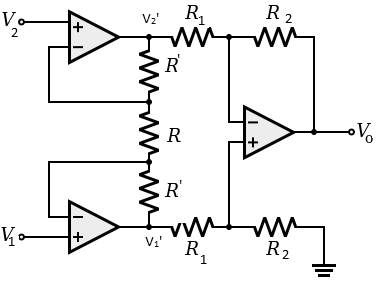
\includegraphics[width=7cm, height=5cm]{IA_DIAGRAM}
	\caption[Figure 1: ]{Instrumentation amplifier}
	\label{fig:IA-CIRCUIT-DIAGRAM}
\end{figure}
	The first stage of the IA consists of two op-amps and acts an input buffer for the second stage, which is a Differential Amplifer with one output.
	\begin{center}The overall gain of this IA circuit is $\frac{R_4}{R_2}\left[1 + \frac{2R_1}{R_{gain}}\right]$.\\\end{center}
	
	Both the inputs are connected directly to the non-inverting inputs of their respective op-amps in the first stage. As the non-inverting input of an op-amp has a very high input impedance due to the nature of the op-amp's internal circuitry, this impedance is high, often in the range of megaohms to gigaohms, depending on the type of op-amp.
	
	(e.g., 1 k$\Omega$ source imbalance, at 60 Hz).\\
	\vspace{.10cm}The term CMR is a logarithmic expression of the 
	common-mode rejection ratio(CMRR).\\ That is, CMR = 
	20 $log_{10}$ CMRR



\section{LITERATURE SURVEY}

		Biomedical signals  are used primarily for extracting information on a biological system under investigation. The process of extracting information could be as simple as measuring the pulse of a person on the wrist or as complex as analyzing the activity of brain neurons.
		
		The primary purpose of a medical device is to measure or determine the presence of some physical quantity that may, in some way, assist the medical personnel to make better diagnosis and treatment.\\
		
		•	\textbf{Measurement Range}:  Generally the measurement ranges are quite low compared with non-medical parameters. Most signals are in the microvolt to millivolt range.\\
		
	For \textit{accurate measurement of voltage}, it is necessary to arrange that the input impedance of the measuring device must be large compared with the output impedance of the signal source. This is to minimize the error that would occur, if an appreciable fraction of the signal source were dropped across the source impedance. Conversely, \textit{accurate measurement of current source signals} necessitates that the source output impedance be large compared with the receiver input impedance. Ideally, a receiver that exhibits a zero input impedance would not cause any perturbation of the current source. Therefore, high-impedance current sources are more easily handled than low-impedance current sources.\\
		
		•	\textbf{Frequency Range}: Most of the bio-medical signals are in the audio frequency range or below and that many signals contain dc and very low frequency components.\\
		
		The frequency response of the system should be compatible with the operating range of the signal being measured. To process the signal waveform without distortion, the bandpass of the system must encompass all of the frequency components of the signal that contribute significantly to signal strength. The range can be determined quantitatively by obtaining a Fourier analysis of the signal.The bandpass of an electronic instrument is usually defined as the range between the upper and lower half-power frequencies
		
		The electrical signals are invariably accompanied by components that are unrelated to the phenomenon being studied. Spurious signal components, which may occur at any frequency within the band pass of the system are known as noise.
		The instruments must be designed in such a way that the noise is minimised to facilitate accurate and sensitive measurement. For extraction of information from noisy signals, it is essential to enhance signal-to-noise(SNR) ratio. The simplest method is that of bandwidth reduction, although many sophisticated methods have been developed to achieve noise reduction from the noisy bio-medical signals. \cite{khandpur2014}
		
		The Instrumentation Amplifier(IA) provides impedance buffering, signal gain and common mode rejection conditions to the selected input signal to a suitable level for application to the ADC.\\
		
		Power vs. Bandwidth, Slew Rate, and Noise :\\
		
			As a general rule, the higher the operating current of the IA's input section, the greater the bandwidth 
			and slew rate and the lower the noise. But higher operating 
			current means higher power dissipation and heat. Hence IC designers often must trade off some specifications to keep power dissipation and drift to acceptable levels
		
\section{DISCUSSION AND ANALYSIS}
 The performance metrics of the designs are summarized in Table 1.

\begin{table}[h!]
\centering
\renewcommand{\arraystretch}{1.2}
\adjustbox{max width=\textwidth}{
\begin{tabular}{|c|c|c|c|c|c|c|c|c|c|c|} 
\hline
\textbf{CMOS TECH} & \textbf{\begin{tabular}[c]{@{}c@{}}Supply \\ Voltage (V)\end{tabular}} & \textbf{\begin{tabular}[c]{@{}c@{}}Gain \\ (dB)\end{tabular}} & \textbf{\begin{tabular}[c]{@{}c@{}}Bandwidth \\ (Hz)\end{tabular}} & \textbf{CMRR} & \textbf{PSRR} & \textbf{NEF} & \textbf{\begin{tabular}[c]{@{}c@{}}INR \\ Vrms\end{tabular}} & \textbf{\begin{tabular}[c]{@{}c@{}}Area \\ (mm\textsuperscript{2})\end{tabular}} & \textbf{\begin{tabular}[c]{@{}c@{}}Power Dissipation \\ ($\mu$W)\end{tabular}} \\ 
\hline
180nm       & 0.9   & 101.61 & 20 -777.5k & 147 & {\begin{tabular}[c]{@{}c@{}}148(+)\\ 154(-)\end{tabular}} & -    & -     & -     & 38.8   \\ 
\hline
TSMC 90nm   & 0.4   & 50     & 14kHz     & 76     & 56   & -    & 3.71  & 0.023 & 11     \\ 
\hline
180nm       & 1     & 35-70  &  800-1400 & 106 & 119 & 0.64 & 0.72 & 0.0625 & 1.85 \\ 
\hline
180nm       & 1.8   & 39.8dB & 6.2kHz    & 105    & -      & 2.24 & -     & -     & 7.79   \\ 
\hline
65nm        & 1.5   & 82     & 145kHz    & 110    & -      & -    & -     & 0.00325$\mu$m\textsuperscript{2} & 6.57$\mu$W \\ 
\hline

\multirow{1}{*}[-7pt]{\centering TSMC 180nm }  & 1.8   & 39.76  & 11.6kHz   & 80     & -      & 3.18 & 3.44        & -     & 25.92  \\ 
                                         & 1   & 39.3   & 5kHz        & 110    & -      & 2.74 & 1.83$\mu$V  & -     & 2.09   \\ 
\hline
1P6M 65nm & 1     & 52.1   & 1-8.200Hz   & {\begin{tabular}[c]{@{}c@{}}90 @100Hz \\ 80 @1kHz \end{tabular}}& 78 & 3.19 & 4.13 & 0.042 & 118$\mu$W \\ 
\hline

{\begin{tabular}[c]{@{}c@{}} BCD 1P6M \\0.18$\mu$m\end{tabular}}& 1.5 & 39.9-59.8 & 1-10kHz & 105 & - & {\begin{tabular}[c]{@{}c@{}}4.05 @1kHz \\ 4.15 @10kHz\end{tabular}} & \begin{tabular}[c]{@{}c@{}}53.9 @11kHz \\ 55.4 @10kHz \\ nV/$\sqrt{\text{Hz}}$
\end{tabular} & - & 3.8$\mu$W \\ 
\hline

\multirow{1}{*}[-7pt]{\centering 0.5$\mu$m }  & \multirow{1}{*}[-7pt]{\centering 1.5 }   & 56.48 & 1.45 kHz   & $>$ 110     & $>$ 100   & 6.5  & 6.44  & -     & 3$\mu$W  \\ 
                                              &                                          & 48.69 & 2.71 Khz   & $>$ 90      & $>$  89   & 4.3  & 4.13  & -     & 6$\mu$W  \\ 
\hline

180nm        & 1.8   & 30 - 40 & 0.05-11Khz  & 84     & 89.3   & 1.92  & 1.34 & 0.03     & 32.94$\mu$W \\ 
\hline
65nm         & 0.4   & 24     & 11kHz     & 83     & -      & -    & -     & 0.00767mm\textsuperscript{2} & 0.089  \\ 
\hline
SCL 180nm    & 0.6   & 61     & 4.1kHz    & -      & -      & -    & 31.5  & -     & 0.086   \\ 
\hline
180          & 1.8 & 34.5 & 1.7-352Hz & 174 & 80 & 2.99 & 3.69 & - & 4.5-19.4 \\ 
\hline
350nm        & 3     & 40     & 550MHz-300Hz & $>$80    & 41     & -    & 7.4   & -     & 20.2   \\ 
\hline
180          & 1.2   & 47     & 1.2MHz    & 98     & 109    & 89n  & -     & -     & 317    \\ 
\hline
TSMC 180     & 1     & 96.41  & 400kHz    & 60     & 153.71 & 610  & -     & -     & 53.72  \\ 
\hline
180          & 1.8   & 79.16  & 9MHz gain BW & 98     & -      & 9.65 & -     & -     & 409.14 \\ 
\hline
TSMC 90      & 0.4   & 41     & 13.5kHz   & 107    & 74.5   & 3.59 & -     & 0.023 & 5.5    \\ 
\hline
TSMC 180     & 0.4   & 28-40  & 2.1 Gain BW & 82     & 60     & -    & -     & 0.064 & 927nW \\ 
\hline
UMC 180nm    & 0.8   & 43     & 1kHz      & 71  & -      & -    & -     & -     & 371    \\ 
\hline
Samsung 130nm & 1    & 55     & 1.1kHz    & 125    & -      & 3.8  & 6.5   & -     & 2.3$\mu$W \\ 
\hline
\end{tabular}
}
\caption{CMOS technology comparison table.}
\label{tab:cmos_table}
\end{table}

\section{CONCLUSION}






%BIBILOGRAPHY%
	
\bibliographystyle{ieeetr}
\bibliography{references}	

	

	


\end{document}

